\styledchapter[Orkestratietools om platformen te beheren]{orkestratietools-om-platformen-te-beheren}
Om resources in een cloud platform te beheren kan gebruik gemaakt worden van een portal. In een portal kan databases, servers en netwerken aangemaakt worden om een infrastructuur te creëren. Omdat een portal uitgebreid en complex is, moet de developer een infrastructuur kunnen opzetten zonder het gebruik van een portal. Dit is mogelijk met \acrfull{iac} orkestratietools. \Acrshort{iac} zal als eerst worden worden uitgelegd. Vervolgens worden verschillende \Acrshort{iac} orkestratietools met elkaar vergeleken. Als laatst wordt een experiment uitgevoerd om de haalbaarheid met een orkestratietool te valideren.

\section{Wat is infrastructure as code?}\label{subsec:ch5-wat-is-infrastructure-as-code}
\acrshort{iac} is een manier om een infrastructuur op te zetten binnen een cloud platform zonder gebruik te maken van een interface zoals een portal. De gewenste infrastructuur wordt beschreven waarna de orkestratietool de gewenste situatie een realiteit probeert te maken \cite{iac-amazon-web-services-in-action}.

De manier waarmee een orkestratietool de infrastructuur aanmaakt, wijzigt of verwijderen is met een plan. In het plan staat welke resources moeten bestaan om aan de gewenste situatie te voldoen. Vaak gaat dit gepaard met configuratie zoals een naam, locatie of tags. In \autoref{fig:ch5-iac-plan-example} is een voorbeeld van een plan te zien. Het plan beschrijf op welke cloud platform dit uitgevoerd moet worden (L12) en wat er aangemaakt moet worden. In dit geval is het een resource group (lijn 16) met als configuratie een naam (\(myTFResourceGroup\)) en locatie (\(westus2\)).

\begin{figure}[hbt!]
  \centering
  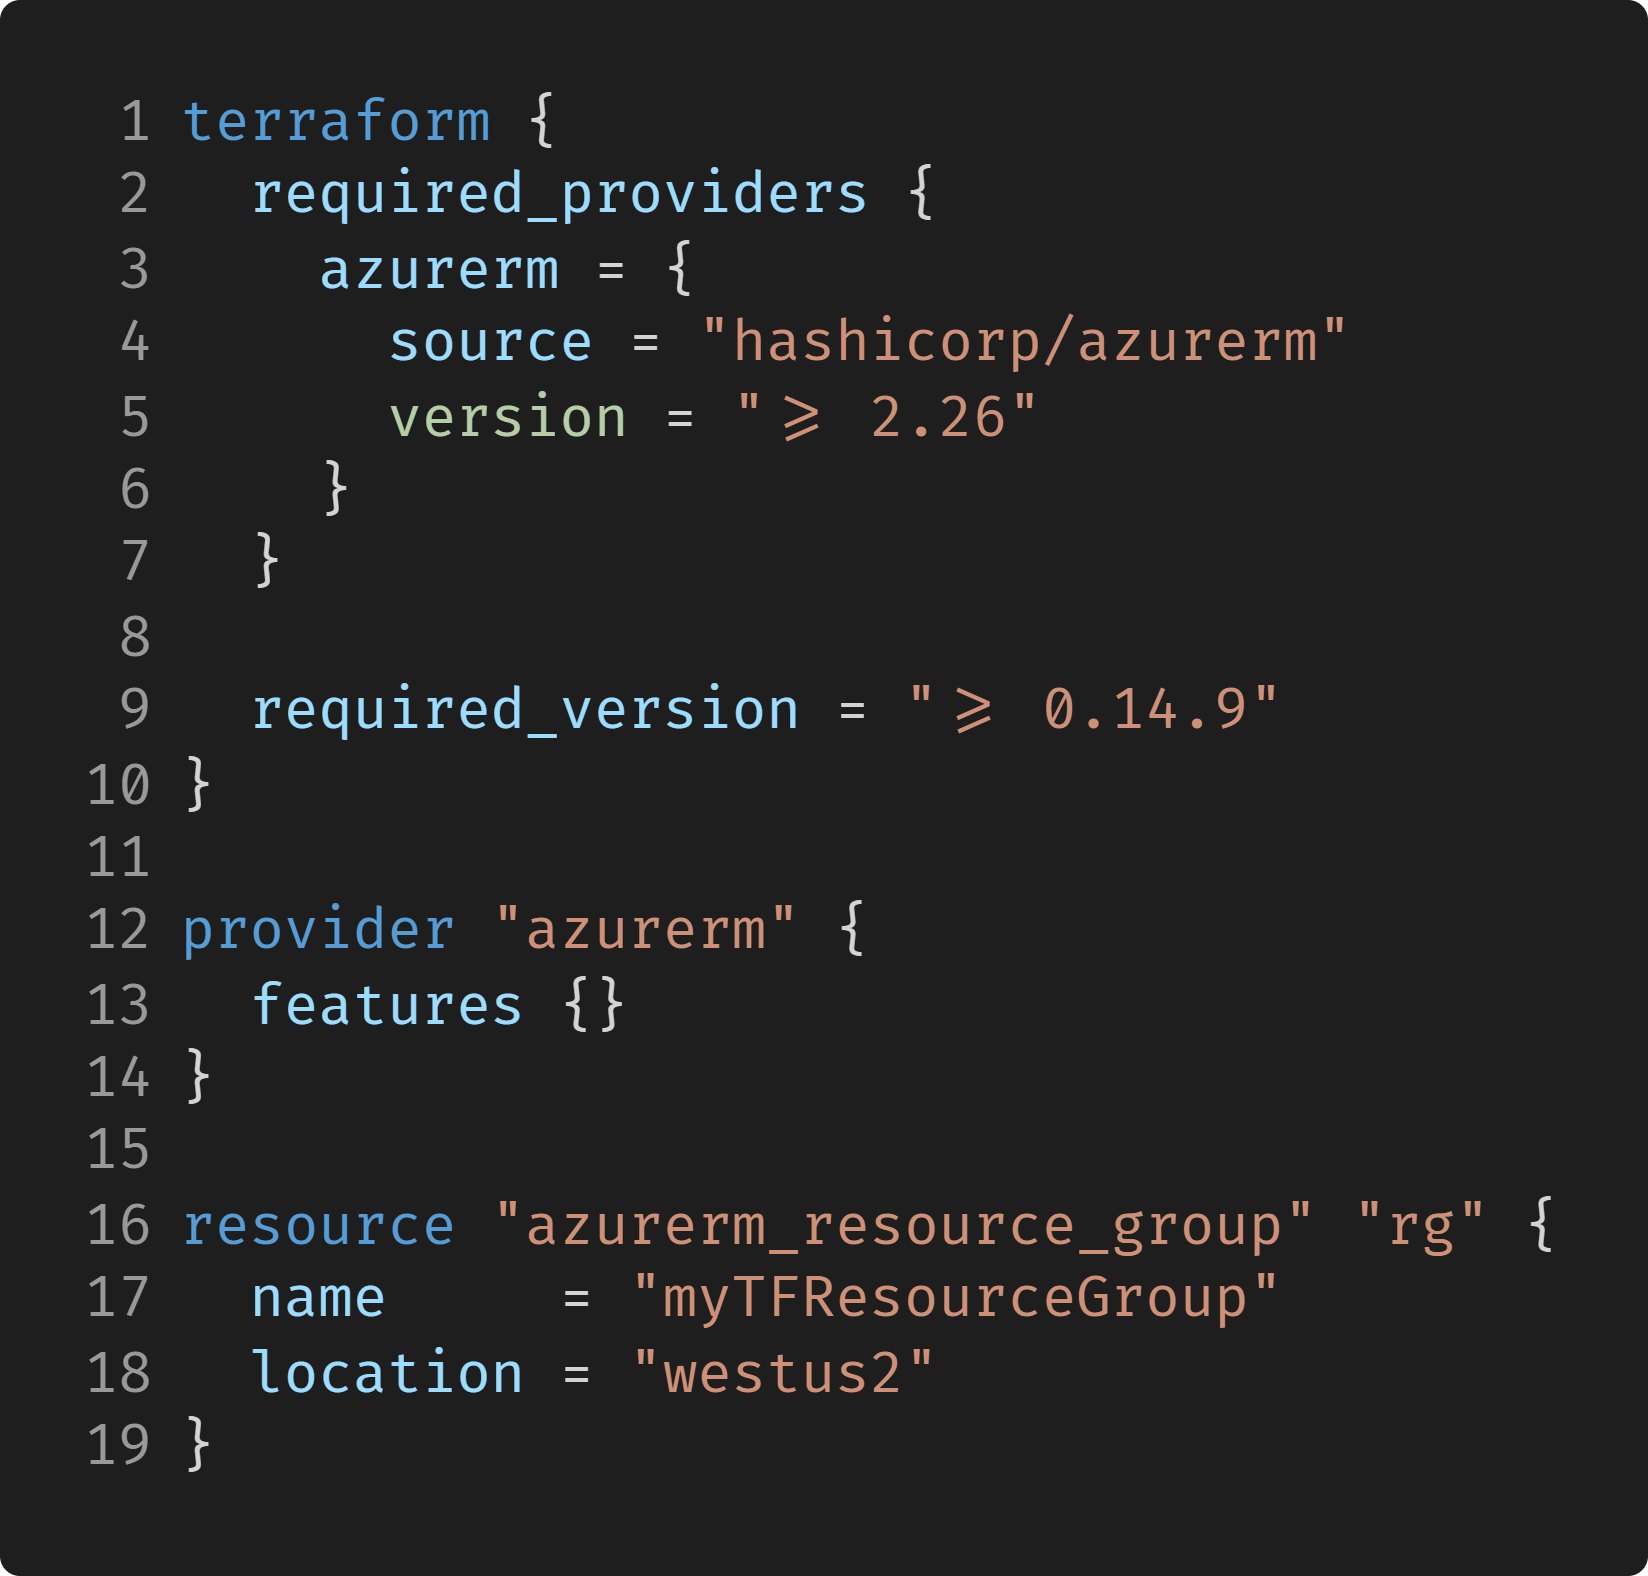
\includegraphics[width=0.5\textwidth]{chapter-5/iac-plan-example.png}
  \caption{Voorbeeld van een \acrfull{iac} plan \cite{terraform-plan-example}.}
  \label{fig:ch5-iac-plan-example}
\end{figure}

Een \Acrshort{iac} volgt een proces om aan de gewenste situatie te voldoen. In \autoref{fig:ch5-iac-process} is te zien hoe een proces verloopt. Zodra de orkestratietool wordt gestart, wordt zowel het plan als de situatie in de cloud platform gecontroleerd en met elkaar vergeleken. In stap 1 is het plan valide, maar de situatie in de cloud platform niet. Dit betekent bijvoorbeeld dat er in het plan staat dat er een resource group moet bestaan met een naam en locatie zoals het beschreven staat in \autoref{fig:ch5-iac-plan-example}, maar dit niet bestaat in de cloud platform. In de volgende stap wordt de resource aangemaakt door de \Acrshort{iac} om aan de gewenste situatie te voldoen. De wijzigingen gebeuren programmatisch en wordt gedaan door de \Acrshort{iac}. Er is geen tussenkomst van een persoon of interface nodig. 

\begin{figure}[hbt!]
  \centering
  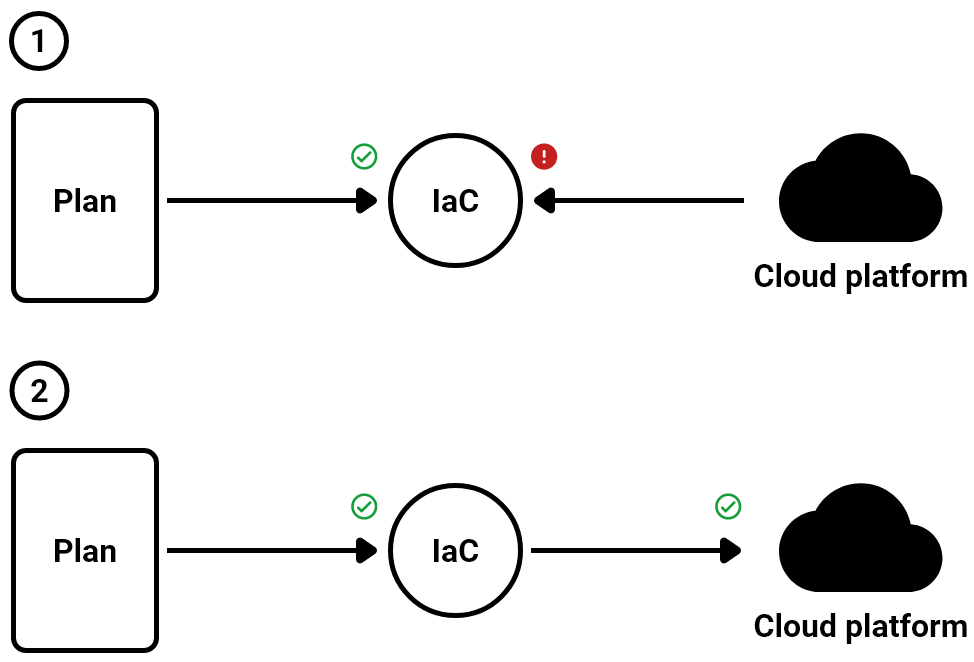
\includegraphics[width=0.75\textwidth]{chapter-5/iac-process.png}
  \caption{Proces van een \acrfull{iac} om aan de gewenste situatie te voldoen.}
  \label{fig:ch5-iac-process}
\end{figure}

\section{Orkestratietools vergeleken met elkaar}\label{subsec:ch5-orkestratietools-vergeleken-met-elkaar}
% Om een keuze te maken met welke \Acrshort{iac} orkestratietool verder gewerkt zal worden moet er een keuze gemaakt worden tussen de orkestratietools die beschikbaar zijn. Om de beschikbaarheid te beperken kan zogenoemde "knockout"\space criteria opgesteld worden. Dit betekent dat een \Acrshort{iac} orkestratietool niet wordt meegenomen in de keuze als de tool niet voldoet aan alle criteria In \autoref{table:knock-out-criteria-orchestration-tools-that-manage-cloud-computing-platformen} zijn de knockout criteria te vinden.

% \begin{table}[hbt!]
%   \centering
%   \begin{tabular}{|p{.2\linewidth}|p{.69\linewidth}|}
%   \hline
%   \textbf{Criteria} & \textbf{Toelichting} \\ \hline
%     Programmatisch beheren
%     &
%     Het framework moet via code een resources kunnen aanmaken, wijzigen en verwijderen. 
%     \\ \hline

%     Ondersteuning voor cloud \newline computing \newline platformen
%     &
%     Om platform-agnostisch te zijn moet de orkestratietool minstens twee cloud computing platformen ondersteunen waarop een ML model getraind kan worden.
%     \\ \hline

%     Uitgebreide \newline documentatie
%     &
%     De documentatie moet toegankelijk en duidelijk zijn. De documentatie moet tutorials, concepten en een reference bevatten.
%     \\ \hline
%   \end{tabular}
%   \caption{Knock-out criteria voor orkestratietools dat cloud computing platformen beheerd.}
%   \label{table:knock-out-criteria-orchestration-tools-that-manage-cloud-computing-platformen}
% \end{table}



% \begin{table}[hbt!]
%   \centering
%   \begin{tabular}{|p{.15\linewidth}|p{.245\linewidth}|p{.245\linewidth}|p{.245\linewidth}|}
%   \hline
%   \textbf{Frameworks} & \textbf{Programmatisch \newline beheren} & \textbf{Ondersteuning voor cloud computing \newline platformen} & \textbf{Uitgebreide \newline documentatie} \\ \hline
%     \textbf{Ansible} &
%     code? &
%     cloud platform ondersteuning &
%     docs
%     \\ \hline

%     \textbf{Pulumi} &
%     code? &
%     cloud platform ondersteuning &
%     docs
%     \\ \hline

%     \textbf{Terraform} &
%     code? &
%     cloud platform ondersteuning &
%     docs
%     \\ \hline
%   \end{tabular}
%   \caption{Knock-out criteria voor orkestratietools dat cloud computing platformen beheerd.}
%   \label{table:orchestration-tools-compared-against-knock-out-criteria}
% \end{table}

% Om verdere afwegingen te maken kan een tweede lijst met criteria opgesteld worden (\autoref{table:criteria-orchestration-tools-that-manage-cloud-computing-platformen}).

% \begin{table}[hbt!]
%   \centering
%   \begin{tabular}{|p{.2\linewidth}|p{.69\linewidth}|}
%   \hline
%   \textbf{Criteria} & \textbf{Toelichting} \\ \hline
%     Ondersteuning voor lokale \newline oplossingen
%     &
%     Naast het ondersteunen van cloud computing platformen moet het framework ook lokale oplossingen zoals Kubernetes of Docker ondersteunen zodat een developer lokaal het model kan trainen [https://www.npmjs.com/package/node-docker-api].
%     \\ \hline
%   \end{tabular}
%   \caption{Criteria voor frameworks dat cloud computing platformen beheerd.}
%   \label{table:criteria-orchestration-tools-that-manage-cloud-computing-platformen}
% \end{table}

\section{Experiment met orkestratietool Pulumi}\label{subsec:ch5-experiment-met-orkestratietool-pulumi}

\section{Conclusie}\label{subsec:ch5-conclusie}


\section{Advies}\label{subsec:ch5-advies}